\documentclass[11pt,a4paper]{book}
\usepackage[utf8]{inputenc}
\usepackage{siunitx}
\usepackage[siunitx]{circuitikz}
\usepackage[english]{babel}
\usepackage{amsmath}
\usepackage{amsfonts}
\usepackage{amssymb}
\usepackage{caption}
\usepackage{subcaption}
\usepackage{pgfplots}
\usepackage{graphicx}
\author{Ege Özkan}
\title{CENG 215 \\ \large{Circuits and Electronics Lecture Notes}}
\begin{document}
\maketitle

\chapter{Introduction - October 15, 2020}


\section{Abstractions}

Recall the Newton's formula $F=ma$, which defines the relationship between force, mass and acceleration. This formula modals acceleration using force and mass. However, according to this model, there is no connection between mass and speed. Consider now, the Einstein's equation:

\begin{equation}
m = \frac{m_0}{\sqrt{1 - \frac{v^2}{c^2}}}
\end{equation}

As this equation shows, speed affects mass. The abstractions ignore certain connections for the sake of simplicity. Likewise, electrical engineering, based on Maxwell's Equations, create abstractions, notably, this lecture deals with the \textit{Lumped Circuit Abstraction}.

Consider a statement in a high level programming language \texttt{int n = 3;}, this basic statment goes through many abstractions eventually reaching circuitery.

\section{Circuits}

\begin{figure}[httb]
\begin{circuitikz} \draw
(0,0) to [V] ++ (2, 0) -- (2,2) to [R] (0, 2) -- (0, 0)
;
\end{circuitikz}
\caption{A simple cirucit abstraction}
\end{figure}


From this abstraction, arises the \textbf{Ohm's Law}

\begin{equation}
v = iR
\end{equation}


\subsection{Two Terminal Element}

\begin{center}
\begin{circuitikz}[american voltages]
\draw
  (0,0) to [short, *-,i_ = $i$] (2,0) 
  to [generic] (2,2) -- (0,2)
  (0, 0)to [open, v^>=$v$, *-] (0,2)
  to [short, *-] (0,2)
;
\end{circuitikz}
\end{center}

Two terminal elements include batteries, resistors, capacitors, etc...

\subsubsection{Battery}

Batteries provide voltage and can be bind into serial or paralel.

\begin{center}
\begin{circuitikz}[american voltages]
\draw
  (0,0) to [short, *-] (2,0)
  to [V, l_=$v$] (2,2) -- (0,2)
  to [short, *-] (0,2)
;
\end{circuitikz}
\end{center}

Below are power (in watts) and energy (in Jouless or watt-seconds) for batteries.

\begin{equation}
P = vi
\label{Power in watt}
\end{equation}

\begin{equation}
w = Pt
\label{Energy formula in joules or watt-seconds}
\end{equation}

Enery formula can also be represented as:

\begin{equation}
w = \int_{t_1}^{t_2} v(t) i(t) \text{d}t
\end{equation}

\subsubsection{Resistance}

\begin{center}
\begin{circuitikz}[american voltages]
\draw
  (0,0) to [short, *-, i_=$i$] (1,0)
  to [tline, l_=$R$] (3,0) to [short, -*] (4,0)
;
\end{circuitikz}
\end{center}

Imagine a generic tube with length $l$, resistivity $\rho$ and cross sectional area $a$, in this case, the Resistance of the element $R$ is

\begin{equation}
R = \rho \frac{l}{a}
\end{equation}

The resistance can be showed as:

\begin{center}
\begin{circuitikz}[american voltages]
\draw
  (0,0) to [short, *-, i_=$i$] (1,0)
  to [R, l_=\text{$R$, $V$}] (3,0) to [short, -*] (4,0)
;
\end{circuitikz}
\end{center}

Where the Ohm's Law state:

\begin{equation}
v = Ri
\end{equation}

or alternativelly

\begin{equation}
i = Gv
\end{equation}

Where $G$ is conductance, whose SI unit is siemens and defined as $\frac{1}{R}$

\subsubsection{Ideal Voltage Source}

Ideal Voltage source can be represnted by:

\begin{center}
\begin{circuitikz}[american voltages]
\draw
  (0,0) to [short, *-] (1,0)
  to [battery1, v<=$v(t)$, i_=$i$] (3,0) to [short, -*] (4,0)
;
\end{circuitikz}
\end{center}

\begin{center}
\begin{circuitikz}[american voltages]
\draw
  (0,0) to [short, *-] (1,0)
  to [V, v<=$v(t)$, i_=$i$] (3,0) to [short, -*] (4,0)
;
\end{circuitikz}
\end{center}

In general, any voltage soucre can be drawn as

\begin{center}
\begin{circuitikz}[american voltages]
\draw
  (0,0) to [short, *-] (2,0)
  to [R, l_ = $r$] (2,2)
  to [V, l_=$v$, i_=$i$] (0,2) 
  to [short, *-] (0,2)
;
\end{circuitikz}
\end{center}

Where $r$ is the internal resistence that arise from the material itself. An ideal voltage source would be able to provide the same current no matter what the voltage is, however this is not possible in real life, where any voltage source has a $r$

\chapter{Resistive Networks - 22 October, 2020}
\begin{figure}[h]
\begin{circuitikz}[american voltages]
\draw (0,2)
	to [short, *-] (-2 , 2)
	to [V, v=10<\volt>, i_=0<\ampere>] (-2,0)
	to [short, -*] (0, 0);
\draw (4, 2)
	to [short, *-] (2, 2)
	to [V, v=10<\volt>, i_=0<\ampere>] (2,0)
	to [short, -*] (4, 0)
	to [R, l_={$\infty$}] (4, 2);
\end{circuitikz}\\
\begin{circuitikz}[american voltages]
\draw (0,2)
	to [short] (-2 , 2)
	to [V, v=10<\volt>, i_=$\infty$] (-2,0)
	to [short] (0, 0)
	to [short] (0, 2);
\draw (4, 2)
	to [short] (2, 2)
	to [V, v=10<\volt>, i_=$\infty$] (2,0)
	to [short] (4, 0)
	to [R, l_={0<\ohm>}] (4, 2);
\end{circuitikz}
\caption{An open circuit is equivalent to a circuit with a resistor with an infinite resistance. Whereas a short cirucit can be modelled as a circuit with zero resistence.}
\end{figure}

The perfect current source is a current source that can supply current in any voltage.


\section{Signals}
\begin{figure}[h]
\begin{subfigure}[b]{\textwidth}
\centering
\begin{tikzpicture}
\begin{axis}
\addplot[domain=0:10, samples=100, color=red]{sin(deg(x))};
\end{axis}
\end{tikzpicture}
\end{subfigure}

\begin{subfigure}[b]{\textwidth}
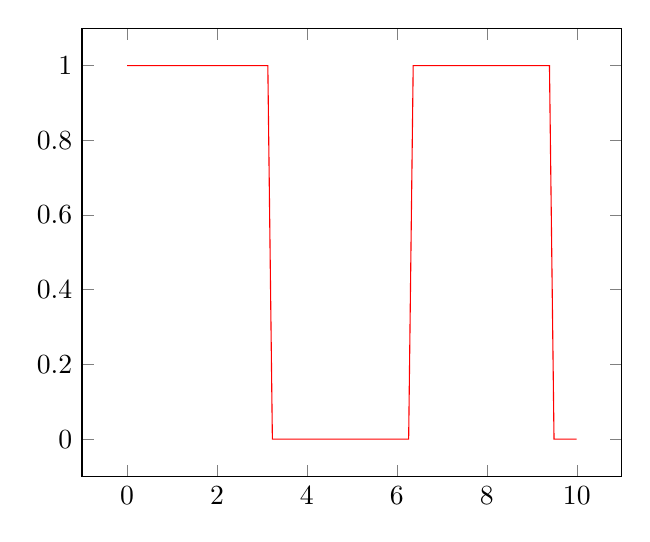
\begin{tikzpicture}
\begin{axis}
\addplot[domain=0:10, samples=100, color=red]{floor(sin(deg(x))) + 1};
\end{axis}
\end{tikzpicture}
\end{subfigure}
\caption{Two signals.}
\label{fig:signals}
\end{figure}

Signals can be analog or digital. In Figure \ref{fig:signals}, the sinosodial signals, which has continous values is an analog signal. Where it is represented via the $v(t) = A\sin(\omega t + \phi)$, where $A$ is its amplitude, $\omega$ is its frequency and $\phi$ is its phase, it is analog because it has \textit{continous} values. In the meantime, the second signal is a digital signal as it has \textit{discrete} and quantised values.\\

Digital signals trade precision about the signal with \textit{immunity towards the noise}.

\begin{description}
\item[Resistance] A measure of the ability of the device to consume energy.
\item[Capacitence] A measure of the ability of the device to store energy in the form of potential energy. (voltage).
\item[Inductance] A measure of the ability of the device to store energy as the moving charge (current).
\end{description}

\section{Resistive Networks}

\begin{center}
\begin{circuitikz}[american voltages]
\draw (2,0)
	to [short] (-2, 0);
\draw (-2, 3)
	to [V^>=$V$] (-2, 0);
\draw (-2, 3)
	to [R=$R_1$, v=$v_1$, i=$i_1$] (2, 3)
	to [R=$R_2$, v=$v_2$, i=$i_2$] (2, 0);
\draw (2, 3)
	to [R=$R_3$, v=$v_3$, i=$i_3$](6, 3)
	to [R=$R_4$, v=$v_4$, i=$i_4$](6, 0)
	to [short] (2, 0);
\end{circuitikz}
\end{center}
This sort of circuits can be analysed using two laws, \textbf{Kirchoff's Current Law} (KCL) and \textbf{Kirchoff's Voltage Law} (KVL).

\subsection{Kirchoff's Current Law}

\begin{center}
\begin{circuitikz}[american voltages]
\draw (2,2)
	to [short, i_=$i_1$] (0,0);
\draw(2, 0)
	to [short, -*, i_=$i_2$] (0, 0);
\draw(2, -2)
	to [short, i_ =$i_3$] (0,0);
\draw(-2, 2)
	to [short, i_=$i_4$](0,0);
\draw(-2, 0)
	to [short, -*, i_=$i_5$] (0, 0);
\draw(-2, -2)
	to [short, i_ =$i_6$] (0,0);
\end{circuitikz}
\end{center}
Kirchoff's current law state that the sum of currents entering a node must equal zero.\\

\begin{equation}
\sum_{n = 1}^6 i_n = 0
\end{equation}

When one takes the directions of the currents into account, this means that the \textit{currents entering a node must equal the curents exiting a node}.

\subsection{Kirchoff's Voltage Law}

\begin{center}
\begin{circuitikz}[american voltages]
\draw (2,0)
	to [short] (-2, 0);
\draw (-2, 3)
	to [V^>=$V_1$] (-2, 0);
\draw (-2, 3)
	to [R=$R_1$, v=$v_1$, i=$i_1$] (2, 3)
	to [R=$R_2$, v=$v_2$, i=$i_2$] (2, 0);
\draw (6, 3)
	to [R=$R_3$, v=$v_3$, i_=$i_3$](2, 3);
\draw(6,3)
	to [V=$V_2$](6, 0)
	to [short] (2, 0);
\end{circuitikz}
\end{center}

Consider three loops, if clockwise, starting from the battery's top, each node is called a, b, c, d then for loop abcda:

\begin{align*}
v_{ba} + v_{bc} + v_{cd} + v_{da} = 0\\
v_{ab} = v_1 = R_1 i_1\\
v_{bc} = v_3 = -R_3 i_3 \\
v_{cd} = V_2\\
v_{da} = -V_1\\
V_2 - V_1 + R_1i_1 -R_3i_3 = 0
\end{align*}

In general, KVL states that, for a closed loop $L$:

\begin{equation}
\sum^{L} v_{L_i} = 0
\end{equation}

That is, sum of voltages in a  closed loop equals to zero.

\subsection{Node Voltage Method}
\begin{center}
\begin{circuitikz}[american voltages]
\draw (2,0)
	to [short] (-2, 0);
\draw (-2, 3)
	to [V^>=32<\volt>] (-2, 0);
\draw (-2, 3)
	to [R=2<\ohm>, i=$i_1$] (2, 3)
	to [R=8<\ohm>, i=$i_3$] (2, 0);
\draw (6, 3)
	to [R=4<\ohm>, i_=$i_2$](2, 3);
\draw(6,3)
	to [V=20<\volt>](6, 0)
	to [short] (2, 0)
	node[ground]{};
\end{circuitikz}
\end{center}

By denoting voltages at nodes as $v_a$, $v_b$, $v_c$ and $v_d$ and connect $v_d$ at the ground, making it effectively zero.\\

\begin{align}
i_1 + i_2 - i_3 = 0 & (\text{  KCL at node b.})\\
i_1 = \frac{v_a - v_b}{2} = \frac{32 - v_b}{2}\\
i_2 = \frac{v_c - v_b}{4} = \frac{20 - v_b}{4}\\
i_3 = \frac{v_b - 0}{8} = \frac{v_b}{8}\\
\end{align}

And therefore subsituting values of $i_1, i_2$ and $i_3$ at Equation 2.3\\

\begin{align*}
\frac{32 - v_b}{2} + \frac{20 - v_b}{4} - \frac{v_b}{8} = 0\\
128 - 4v_b + 40 - 2v_b - v_b = 0\\
v_b = 24\text{V}
\end{align*}

And from here, one can calculate the currents.

\begin{align*}
i_1 = \frac{32 - 24}{2} = \text{ 4A}\\
i_2 = \frac{20 - 24}{4} = \text{ 1A}\\
i_3 = \text{ 3A}\\
\end{align*}

\begin{circuitikz}
\draw (0,0)
	to [battery, v^>=5<\volt>] (0, 6)
	to [short] (4, 6)
	to [R=1<\kilo\ohm>] (4, 4)
	to [R=1<\kilo\ohm>] (4, 2)
	to [R=1<\kilo\ohm>] (4, 0)
	to [short] (0, 0);
\end{circuitikz}

\end{document}